%%%%%%%%%%%%%%%%%%%%%%%%%%%%%%%%%%%%%%%%%
% Journal Article
% LaTeX Template
% Version 1.4 (15/5/16)
%
% This template has been downloaded from:
% http://www.LaTeXTemplates.com
%
% Original author:
% Frits Wenneker (http://www.howtotex.com) with extensive modifications by
% Vel (vel@LaTeXTemplates.com)
%
% License:
% CC BY-NC-SA 3.0 (http://creativecommons.org/licenses/by-nc-sa/3.0/)
%
%%%%%%%%%%%%%%%%%%%%%%%%%%%%%%%%%%%%%%%%%

%----------------------------------------------------------------------------------------
%	PACKAGES AND OTHER DOCUMENT CONFIGURATIONS
%----------------------------------------------------------------------------------------

\documentclass[]{article}

\usepackage{blindtext} % Package to generate dummy text throughout this template 

\usepackage[sc]{mathpazo} % Use the Palatino font
\usepackage[T1]{fontenc} % Use 8-bit encoding that has 256 glyphs
\linespread{1.05} % Line spacing - Palatino needs more space between lines


\usepackage[english]{babel} % Language hyphenation and typographical rules

\usepackage[hmarginratio=1:1,top=15mm,left= 10mm, right=10mm, bottom= 8mm]{geometry} % Document margins
\usepackage[hang, small,labelfont=bf,up,textfont=it,up]{caption} % Custom captions under/above floats in tables or figures
\usepackage{booktabs} % Horizontal rules in tables

\usepackage{lettrine} % The lettrine is the first enlarged letter at the beginning of the text

\usepackage{enumitem} % Customized lists
\setlist[itemize]{noitemsep} % Make itemize lists more compact
\usepackage[dvips]{graphicx}
\graphicspath{{noiseimages/}}
\usepackage{listings}
\usepackage{color}
\usepackage{multirow}
\usepackage{longtable}
\usepackage{xcolor}
\usepackage{hyperref}
\definecolor{linkcolor}{HTML}{799B03} % цвет ссылок
\definecolor{urlcolor}{HTML}{799B03} % цвет гиперссылок

\hypersetup{pdfstartview=FitH,  linkcolor=linkcolor,urlcolor=urlcolor, colorlinks=true}
\makeatletter
\newcommand{\setword}[2]{%
	\phantomsection
	#1\def\@currentlabel{\unexpanded{#1}}\label{#2}%
}
\makeatother


% Define Language
\lstdefinelanguage{Protobuf}
{
	% list of keywords
	morekeywords={
		int32,
		message,
		enum,
		double,
		string,
		required
	},
	sensitive=false, % keywords are not case-sensitive
	morecomment=[l]{//}, % l is for line comment
	morecomment=[s]{/*}{*/}, % s is for start and end delimiter
	morestring=[b]" % defines that strings are enclosed in double quotes
}

\usepackage{abstract} % Allows abstract customization
\renewcommand{\abstractnamefont}{\normalfont\bfseries} % Set the "Abstract" text to bold
\renewcommand{\abstracttextfont}{\normalfont\small\itshape} % Set the abstract itself to small italic text

\usepackage{titlesec} % Allows customization of titles
%\renewcommand\thesection{\Roman{section}} % Roman numerals for the sections
%\renewcommand\thesubsection{\roman{section}} % roman numerals for subsections
\titleformat{\section}[block]{\Large\scshape}{\thesection.}{1em}{} % Change the look of the section titles
%\titleformat{\subsection}[block]{\large}{\thesubsection.}{1em}{} % Change the look of the section titles

%\usepackage{fancyhdr} % Headers and footers
%\pagestyle{fancy} % All pages have headers and footers
%\fancyhead{} % Blank out the default header
%\fancyfoot{} % Blank out the default footer
% Custom header text
%\fancyfoot[RO,LE]{\thepage} % Custom footer text
\pagestyle{empty} 

\usepackage{titling} % Customizing the title section

\usepackage{hyperref} % For hyperlinks in the PDF

%----------------------------------------------------------------------------------------
%	TITLE SECTION
%----------------------------------------------------------------------------------------

\setlength{\droptitle}{-3\baselineskip} % Move the title up

\pretitle{\begin{center}\huge\bfseries} % Article title formatting
\posttitle{\end{center}} % Article title closing formatting
\title{Telemetry for getting statistics for which features are used the most in Krita} % Article title

\begin{document}
%\date{}
\maketitle
\section{Contact Information}
\textbf{Full name:}~~~~~~~~~~~~~~~~~Alexey Kapustin \\
\textbf{Email:}~~~~~~~~~~~~~~~~~~~~~~~~djkah11@yandex.com \\
\textbf{IRC nickname:      }~~~~~~~~~akap \\
\textbf{Telegram nickname: }~aluka1 \\
\textbf{Phone: }~~~~~~~~~~~~~~~~~~~~~~8-999-986-73-81 \\
\textbf{Location:          }~~~~~~~~~~~~~~~~~~Moscow, Russia
\section{Problem}
Krita contains a large number of tools for painters, a large number of settings and features.
Their number increases every year, but not all of them are popular. More precisely, the critics want to know which of the options are popular. Based on this information, you can determine the vector of further work, finalize popular, but not too well-implemented features, remove old, useless functions. Use of clickstream analytics will help to learn the popularity of feautures.

The collection of statistics will help to create  achievements to the Steam. Achievements for Krita is good marketing solution, which help us to find new users. It would be reasonable to make two versions: Steam version and non-Steam version. All the information sent will be completely anonymous for the non-Steam version , and will also be collected with direct user's permission . For users of the Steam version, the collected information necessary to achievements, will be associated with their steam-profiles.

%\begin{itemize}
%\item Donec dolor arcu, rutrum id molestie in, viverra sed diam
%\item Curabitur feugiat
%\item turpis sed auctor facilisis
%\item arcu eros accumsan lorem, at posuere mi diam sit amet tortor
%\item Fusce fermentum, mi sit amet euismod rutrum
%\item sem lorem molestie diam, iaculis aliquet sapien tortor non nisi
%\item Pellentesque bibendum pretium aliquet
%\end{itemize}
%\blindtext % Dummy text
%Text requiring further explanation\footnote{Example %footnote}.
\section{Implementation}
\subsection{Client-side}
The main idea is to use Google Protobuf logs to write out necessary information. All information is stored in the logs and as necessary (too large log file, not sent for a long time, etc.) is sent to the server. Sending in the original form the information is irrational, so before sending, the information from the log is analyzed and only the "squeeze" from this information is sent to the server.\\
Main data that we want to analyze:




%\centering
\begin{longtable}{|c|c|l|}
\hline
Information about & Source & Data \\
\hline \hline

Tools & \begin{tabular}[x]{@{}c@{}}KisTool::activate, KisTool:deactivate,\\etc, overloaded in specific tools\end{tabular}
 &\begin{lstlisting}[language=Protobuf]
int32 activationTime;
int32 useTime;
int32 kindTool;
\end{lstlisting} \\
\hline 
\hline \hline
Presets & KisToolFreehandHelper::initPaintImpl &
    \begin{lstlisting}[language=Protobuf,escapechar=|]
string koid;
double paintOpFlow;
string compositeMode;
double savedBrushSize;
int32  hashCode;[|\ref{Word:ref1}|]
	\end{lstlisting} \\
	\hline \hline
	Actions & KisMainWindows actioncollection() &
	\begin{lstlisting}[language=Protobuf,escapechar=|]
string name;
string actionSource;[|\ref{Word:ref2}|]
	\end{lstlisting} \\
	\hline \hline
	Image\_Properties & KisDocument::saveFile &
	\begin{lstlisting}[language=Protobuf,escapechar=|]
int32 fileFormat;
int32 colorSpace;
string colorProfile;
int32 imageSize;
int32 width;
int32 height;
int32 numLayers;
	\end{lstlisting} \\
	\hline \hline
	Asserts & kis\_assert\_common() &
	\begin{lstlisting}[language=Protobuf,escapechar=|]
string assertMessage;
string file;
int32 line;
	\end{lstlisting} \\
	\hline
	

\end{longtable}
~~~~~~~~~~~~~~~~~[\setword{1}{Word:ref1}]: It is required to save presets into map structure for less size of log.
 [\setword{2}{Word:ref2}]: Hotkey, menu of something else\\

\subsection{Server-side}
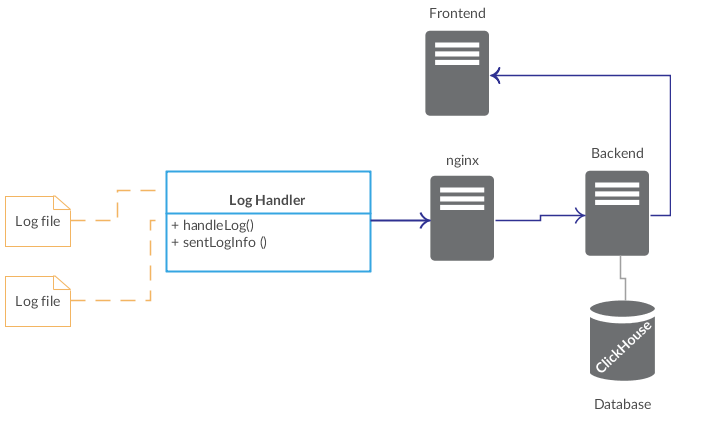
\includegraphics[scale=0.8]{scheme}
\subsubsection{Own stats}
Unfortunately, clickstream services are focused on gathering information from websites. Own implementation allows you to create a convenient api for yourself, and also leaves room for further development and expansion.\\
Scheme description:
The data from the user is serialized and sent to our nginx, which proxy requests to the backend.On the backend, there is deserialization and recording of information in the database.  The information from the database returns to the backend, where it then goes to the front-line. This scheme seems somewhat redundant, but it has an extensible architecture and is capable of withstanding highloads. Nginx is  an optional element, but with increasing load, this architecture will allow you to scale horizontally
\subsubsection{Steam achivments}
It is required to add Steam Sdk.We should to create achievements via Steam web interface. Filling in the list of achievements will be discussed with community. Before any functions can be used, first  {\itshape SteamAPI\_Init()} must be called.After that we can call \textit{SteamUserStats()->SetAchievement( "Draw\_the\_length\_of\_the\_equator") }and set specific achivment.
\subsection{Example}
Here is an example of how data storage for a class will be implemented.KisTelemetryTools is singleton.\\
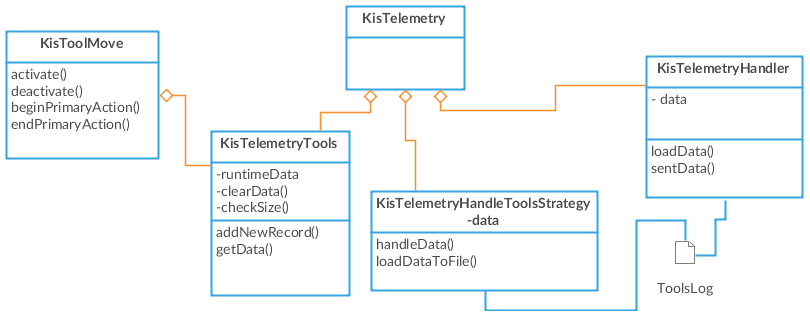
\includegraphics[scale=0.8]{Tools_uml4}\\
When events triggered by KisToolMove::activate, KisToolMove::beginPrimaryAction, KisToolMove::endPrimaryAction, information is written to the appropriate structure in.When the KisToolMove::deactivate event triggers, information from this structure about usage will be sent to the class KisTelemetryTools. When a certain size is reached, the information stored in KisTelemtryTools::runtimeData is passed to KisTelemetryHandleToolsStrategy, where it is processed and loaded into a file. For example, we have 10 records that KisToolMove was used (one entry is one use interval between KisToolMove::activate() and KisToolMove::deactivate()). This information is analyzed, serialized and written to a file. Record: total usage time, average usage time, average time between activation and deactivation, total time between excitation and deactivation, number of uses (10), name of this tool. It is reasonable to replace the name of the tool with some number to save memory.When Krita is completed, KisTelemetryHandler is called. It reads the file(s) and tries to send it to the server. All data is transmitted over the https protocol.
We have a post-request that looks like this (request body):
\begin{lstlisting}[language=XML]
{
"avgUseTime": 111,
"avgADtime": 222,
"useTime": 333,
"useAdTime": 444,
"useCount": 10,
"toolName": 1
}
\end{lstlisting} 
The request comes to nginx whence it is proxied to the backend-server. Comes to the backend server, deserialized, checked for correctness. After that, it records the database in approximately this way. The frontend periodically polls the backend and, based on the state of the database, issues current statistics "online".
\subsection{Technologies}
Protocol Buffers (a.k.a., Google protobuf) are Google's language-neutral, platform-neutral, extensible mechanism for serializing structured data. 
For C++ language it provides a runtime multi-platform library. Nginx is widespread server, which is used by nearby 70\% percents of top-100 worldwide side. ClickHouse allows you to perform analytical queries interactively on real-time data. The system is scalable to very large amounts of data. 



\section{Timeline}


\begin{longtable}{l l}

		\begin{minipage}[t]{0.4\paperwidth}
			\begin{tabular}[t]{|l|l|} % <--- "[t]" is new
			\hline
			\multicolumn{2}{|c|}{Work schedule}\\ \hline
			Period & Work\\
			\hline 22 May - 4 June  &
			\begin{tabular}[x]{@{}l@{}}End of the academic year. I can\\ to work 7-10 hours per week.\end{tabular}
			\\ \hline
			4 June - 18 June &
			\begin{tabular}[x]{@{}l@{}}Exams in university. I can start\\ working 25-30 hours
				per week.\end{tabular} \\
			\hline
			18 June - 29 Aug. &
			\begin{tabular}[x]{@{}l@{}}  During this period I can work \\full-time on the project.\end{tabular}\\
	
				\hline
				29 June - 15 Sept. &
				\begin{tabular}[x]{@{}l@{}}  During this period I can work \\full-time on the project and this \\ period serves as
					compensation \\for the first periods.\end{tabular}\\
				\hline
			\end{tabular}
		\end{minipage}
		&
		
			\begin{minipage}[t]{0.4\paperwidth}
				\begin{tabular}[t]{|l|l|} % <--- "[t]" is new
					\hline
					\multicolumn{2}{|c|}{Implementation timeline}\\ \hline
					Period & Work\\
					\hline 22 May - 4 June  &
					\begin{tabular}[x]{@{}l@{}}I study a code of a client part, \\ I begin to do system of logging.\end{tabular}
					\\ \hline
					4 June - 15 June &
					\begin{tabular}[x]{@{}l@{}}Impelementing logging system for tools.\end{tabular} \\
					\hline
					15 June - 29 June. &
					\begin{tabular}[x]{@{}l@{}} Impelementing logging system for\\ asserts and Image\_Properties\\
						without taking care of memory.\\ Unstable work is possible\end{tabular}\\
					
					\hline
					29 June - 20 Jul. &
					\begin{tabular}[x]{@{}l@{}}  
						End of the implementation of the\\ logging system. Memory optimizations.\\
						Investigate communication between\\ server and client
						\end{tabular}\\
					\hline
					20 Jul - 1 Aug. &
					\begin{tabular}[x]{@{}l@{}}  
						Creation of Steam-version.
						Discussion \\ of achievements with community.
					\end{tabular}\\
					\hline
						1 Aug - 29 Aug. &
						\begin{tabular}[x]{@{}l@{}}  
							Creation of server-side. Load testing.
						\end{tabular}\\
						\hline
							29 Aug - 15 Sept. &
							\begin{tabular}[x]{@{}l@{}}  
								Buffer time for issues\\ that may take longer
								than expected.
							\end{tabular}\\
							\hline
				\end{tabular}
			\end{minipage}
			\\
		\end{longtable}
		%-----------------------
\section{About me}
I'm Alexey Kapustin, a 3rd year student of Bauman Moscow State Technical University of Software Engineering 
Faculty. I'm interested in C ++, Python,Javascript, web development. I also study at the Technopark Mail.ru in the 3rd semester. (Russian School of Web Architects).
\\ 
I did projects using Django, Nodejs.
Within the semester project in the second year of education, I made a simple tower-defense game on SFML C++ library. In the third year I made an API for working with the "Forums" database, which withstood high loads. To create this api, I used the libraries Wt, Qt, Libzdb.
 Since last summer I have commited  to Krita. You can also see my \href{https://github.com/akapust1n}{githab}.




%------------------------------------------------




\end{document}
